%----------------------------------------------------------------------------------------
%    PACKAGES AND THEMES
%----------------------------------------------------------------------------------------

\documentclass[aspectratio=169,xcolor=dvipsnames]{beamer}
\usetheme{SimplePlus}

\usepackage{hyperref}
\usepackage{graphicx} % Allows including images
\usepackage{booktabs} % Allows the use of \toprule, \midrule and \bottomrule in tables
\usepackage{tikz}
\usepackage{cite}
\usepackage{bibentry}
\usepackage[sort,numbers]{natbib}
\usepackage{algorithm, algpseudocode}
\usepackage{amssymb}
\usepackage[overridenote]{pdfpc}

\makeatletter
\providecommand{\bigsqcap}{%
  \mathop{%
    \mathpalette\@updown\bigsqcup
  }%
}
\newcommand*{\@updown}[2]{%
  \rotatebox[origin=c]{180}{$\m@th#1#2$}%
}
\makeatother
\setbeamertemplate{footline}[text line]{%
  \parbox{\linewidth}{\vspace*{-8pt}\insertsectionhead\hfill\usebeamertemplate{page number in head/foot}}}
\setbeamertemplate{navigation symbols}{}

\nobibliography* 

%----------------------------------------------------------------------------------------
%    TITLE PAGE
%----------------------------------------------------------------------------------------

\title{Static Program Analysis For Security}
\subtitle{Cambridge IB Tech Talks}

\author{Zayne Zhang}

\institute{zz513@cam.ac.uk}
\date{March 12, 2025}

%----------------------------------------------------------------------------------------
%    PRESENTATION SLIDES
%----------------------------------------------------------------------------------------

\begin{document}

\begin{frame}
	% Print the title page as the first slide
	\titlepage
\end{frame}

\begin{frame}{Overview}
	% Throughout your presentation, if you choose to use \section{} and \subsection{} commands, these will automatically be printed on this slide as an overview of your presentation
	\tableofcontents
\end{frame}

%------------------------------------------------
\section{Introduction to Static Program Analysis}
%------------------------------------------------

\begin{frame}{How to find bugs in code?}

	{\bf Dynamic Analysis (e.g. Unit Testing, Fuzzing)}
	\begin{itemize}
		\item Done on a limited number of different inputs
		\item Often reveals the presence of errors but {\bf cannot guarantee their absence}
		\item 100\% test coverage != bug-free code
		\item Many tests are regressive and only added after a bug is found
	\end{itemize} \bigskip
	{\bf Static Analysis: analyze code without executing it}
	\begin{itemize}
		\item Can check all possible executions and provide guarantees about its behavior
		\item With the right tools, can catch bugs early in the development process
		\item Particularly useful for testing the absence of security vulnerabilities
	\end{itemize}
\end{frame}

%------------------------------------------------

\begin{frame}{How to find bugs in code?}
	\note{Shows that 1. you can never trust QA engineers and 2. you can never ancitipate
		everything that happens in the real world.}
	\begin{figure}
		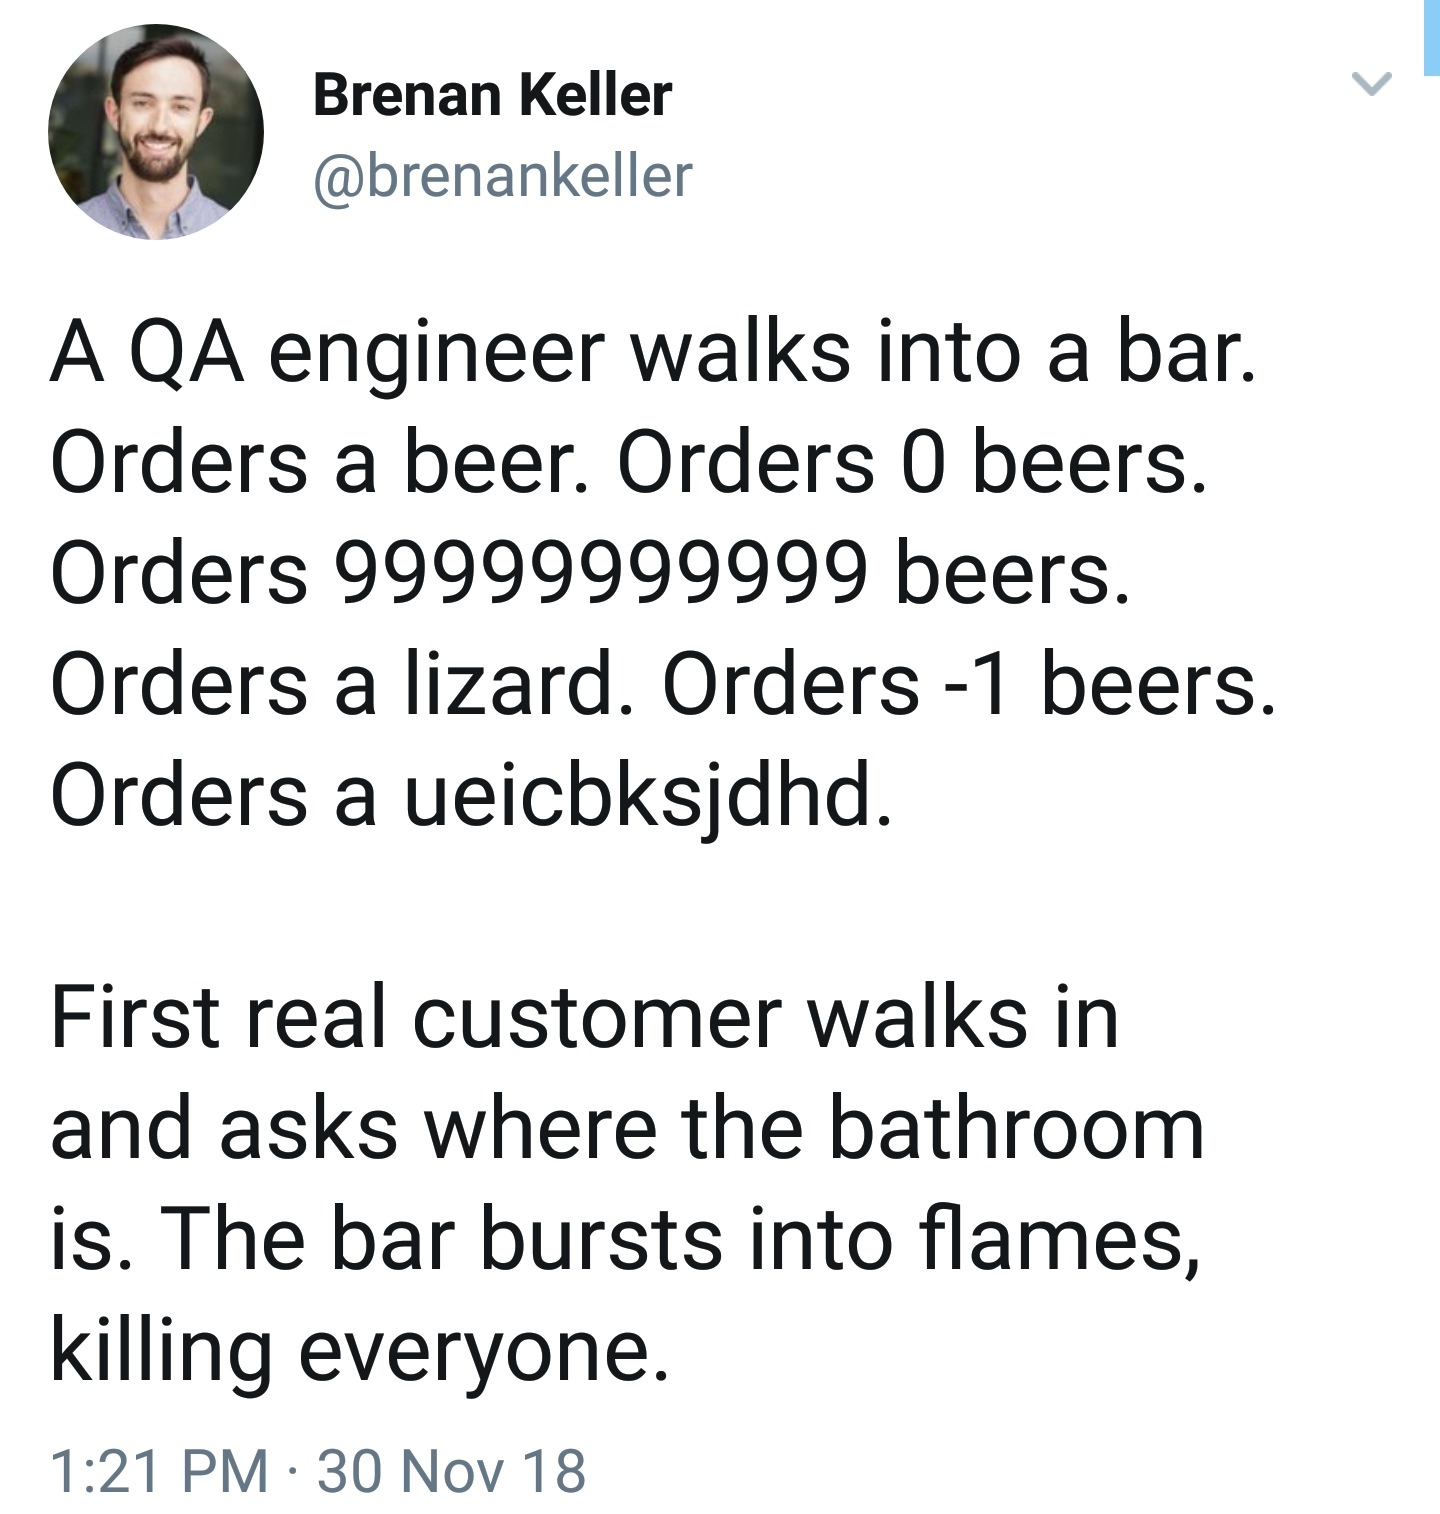
\includegraphics[height=0.8\textheight]{img/1.jpeg}
	\end{figure}
\end{frame}

%------------------------------------------------

\begin{frame}{Data Flow Analysis}
	A particular form of static analysis that {\bf examines how data moves through a program} to answer questions such as:
	\begin{itemize}
		\item What values can reach this point in the code?
		\item Is this variable always initialized before it is used?
		\item \alert{\bf Does untrusted data ever reach an unsafe function?}
	\end{itemize}
\end{frame}

%------------------------------------------------
\section{Lattices and Fixed Points}
%------------------------------------------------

\begin{frame}{Partial Orders}
	\begin{definition}
		A {\bf partial order} $(S, \sqsubseteq)$ is a set $S$ equipped with a binary relation
		$\sqsubseteq$ that is:
		\begin{itemize}
			\item {\bf Reflexive}: $\forall x \in S, x \sqsubseteq x$
			\item {\bf Transitive}: $\forall x, y, z \in S, x \sqsubseteq y \land y \sqsubseteq z
				      \Rightarrow x \sqsubseteq z$
			\item {\bf Antisymmetric}: $\forall x, y \in S, x \sqsubseteq y \land y \sqsubseteq x
				      \Rightarrow x = y$
		\end{itemize}
	\end{definition}

	\begin{itemize}
		\item $y \in S$ is an upper bound for $X$ ($X \sqsubseteq y$) if $\forall x \in X, x \sqsubseteq y$
		\item $y \in S$ is the least upper bound for $X$ ($X \bigsqcup y$) if $y$ is an upper bound for $X$ and $\forall z \in S, X \sqsubseteq z \Rightarrow y \sqsubseteq z$
		\item $y \in S$ is a lower bound for $X$ ($y \sqsubseteq X$) if $\forall x \in X, y \sqsubseteq x$
		\item $y \in S$ is the greatest lower bound for $X$ ($y \bigsqcap X$) if $y$ is a lower bound for $X$ and $\forall z \in S, z \sqsubseteq X \Rightarrow z \sqsubseteq y$
	\end{itemize}

\end{frame}

%------------------------------------------------

\begin{frame}{Lattices}
	\begin{definition}
		A {\bf lattice} $(L, \sqsubseteq)$ is a partial order $(L, \sqsubseteq)$ in which
		every pair of elements $x, y \in L$ has a least upper bound $x \sqcup y$ (join)
		and a greatest lower bound $x \sqcap y$ (meet). \bigskip

		A {\bf complete lattice} is a lattice in which every subset has a least upper bound
		and a greatest lower bound.
	\end{definition}
\end{frame}

%------------------------------------------------

\begin{frame}{Sign Analysis}
	\note{Complete lattice because every two nodes have converging paths in both directions.}

	As an example, we want to find the possible signs of integer variables and
	expressions.

	Consider the following abstract values for the sign of an integer:

	\begin{columns}[c] % The "c" option specifies centered vertical alignment while the "t" option is used for top vertical alignment

		\column{.45\textwidth} % Left column and width
		\begin{itemize}
			\item $\top$: unknown sign
			\item $+$: positive
			\item $-$: negative
			\item $0$: zero
			\item $\bot$: not an integer, or unreachable code
		\end{itemize}

		\column{.45\textwidth} % Right column and width

		\begin{center}
			\begin{tikzpicture}[scale=1.3]
				\node (top) at (0,1) {$\top$};
				\node (minus) at (-1,0) {$-$};
				\node (plus) at (1,0) {$+$};
				\node (zero) at (0,0) {$0$};
				\node (bot) at (0,-1) {$\bot$};

				\draw [<-](top) -- (minus);
				\draw [<-](top) -- (plus);
				\draw [<-](top) -- (zero);
				\draw [<-](minus) -- (bot);
				\draw [<-](plus) -- (bot);
				\draw [<-](zero) -- (bot);
			\end{tikzpicture}
		\end{center}

		This partial order, with edges for $\sqsubseteq$, forms a complete lattice.
		e.g. $+ \sqsubseteq \top$ means $+$ is {\it at least as precise} as $\top$

	\end{columns}
\end{frame}

%------------------------------------------------

\begin{frame}[fragile]{Sign Analysis}
	\note{The map lattice is also a complete lattice. Can intuitively see that you can
		define the partial order by an element-wise comparison of the signs of each variable.}

	Let's create a {\bf map lattice} {\it State = Var $\rightarrow$ Sign} that describes the sign of
	each variable. Derive a system of equations, one per line, using values from
	the lattice.

	\begin{columns}[c] % The "c" option specifies centered vertical alignment while the "t" option is used for top vertical alignment

		\column{.45\textwidth} % Left column and width
		\begin{verbatim}
			var a, b;					// 1
			a = 42;						// 2
			b = a + input(); 	// 3
			a = a - b;				// 4
		\end{verbatim}
		\begin{align*}
			x_1 & = [a \mapsto \top, b \mapsto \top] \\
			x_2 & = x_1[a \mapsto +]                 \\
			x_3 & = x_2[b \mapsto x_2(a) + \top]     \\
			x_4 & = x_3[a \mapsto x_3(a) - x_3(b)]
		\end{align*}

		\column{.45\textwidth} % Right column and width

		\begin{center}
			\begin{tikzpicture}[scale=1.4]
				\node (top) at (0,1) {$\top$};
				\node (minus) at (-1,0) {$-$};
				\node (plus) at (1,0) {$+$};
				\node (zero) at (0,0) {$0$};
				\node (bot) at (0,-1) {$\bot$};

				\draw [<-](top) -- (minus);
				\draw [<-](top) -- (plus);
				\draw [<-](top) -- (zero);
				\draw [<-](minus) -- (bot);
				\draw [<-](plus) -- (bot);
				\draw [<-](zero) -- (bot);
			\end{tikzpicture} \bigskip

			{\it Sign}
		\end{center}
	\end{columns}
\end{frame}

%------------------------------------------------

\begin{frame}[fragile]{Sign Analysis}
	\note{Each abstract state depends on other abstract states, and we can encode these
		as functions.}

	\begin{columns}[c] % The "c" option specifies centered vertical alignment while the "t" option is used for top vertical alignment

		\column{.45\textwidth} % Left column and width
		\begin{align*}
			x_1 & = [a \mapsto \top, b \mapsto \top] \\
			x_2 & = x_1[a \mapsto +]                 \\
			x_3 & = x_2[b \mapsto x_2(a) + \top]     \\
			x_4 & = x_3[a \mapsto x_3(a) - x_3(b)]
		\end{align*}

		\column{.45\textwidth} % Right column and width
		\begin{align*}
			f_1(x_1, \ldots, x_n) & = [a \mapsto \top, b \mapsto \top] \\
			f_2(x_1, \ldots, x_n) & = x_1[a \mapsto +]                 \\
			f_3(x_1, \ldots, x_n) & = x_2[b \mapsto x_2(a) + \top]     \\
			f_4(x_1, \ldots, x_n) & = x_3[a \mapsto x_3(a) - x_3(b)]
		\end{align*}
	\end{columns} \bigskip

	Generalised equation system over a lattice $L$, with functions $f_i: L^n
		\rightarrow L$:
	\begin{align*}
		x_1 & = f_1(x_1, \ldots, x_n) \\
		x_2 & = f_2(x_1, \ldots, x_n) \\
		\vdots                        \\
		x_n & = f_n(x_1, \ldots, x_n)
	\end{align*}
\end{frame}

%------------------------------------------------

\begin{frame}{Monotonicity and Fixed Points}
	\note{If we combine all the functions into one, we are essentially solving for
		$x = F(x)$.}

	Generalised equation system over a lattice $L$, with functions $f_i: L^n
		\rightarrow L$:
	\begin{align*}
		x_1 & = f_1(x_1, \ldots, x_n) \\
		x_2 & = f_2(x_1, \ldots, x_n) \\
		\vdots                        \\
		x_n & = f_n(x_1, \ldots, x_n)
	\end{align*}

	Combine the $n$ functions into $F: L^n \rightarrow L^n$:
	\begin{align*}
		F(x_1, \ldots, x_n) & = (f_1(x_1, \ldots, x_n), \ldots, f_n(x_1, \ldots, x_n)) \\
		                    & = (x_1, \ldots, x_n)
	\end{align*}

	Then we are looking for $x = F(x)$, i.e. a fixed point of $F$.
\end{frame}

%------------------------------------------------

\begin{frame}{Monotonicity and Fixed Points}
	\note{Intuitively, the more we know about the variables at each point, the more we
		know about the variables at the next point.}
	\note{We can always find a unique solution to the equation system.}

	\begin{definition}
		A function $f: L_1 \rightarrow L_2$ is {\bf monotone} if $\forall x, y \in L_1, x \sqsubseteq y \Rightarrow$$ f(x)
		\sqsubseteq f(y)$
	\end{definition}

	{\it More precise input leads to more precise output}

	\begin{theorem}
		{\bf Kleene's Fixed Point Theorem}: In a complete lattice $L$ with finite height,
		every monotone function $f: L \rightarrow L$ has a unique least fixed point
		$\bigsqcup_{i=0}^{\infty} f^i(\bot)$
	\end{theorem}

	These results generalise to functions that take multiple arguments $f: L^n
		\rightarrow L$ that are monotone in each argument -- such as the ones we
	derived for sign analysis.

	\begin{corollary}
		For an equation system over complete lattices of finite height with monotone constraint functions,
		{\bf a unique, most precise solution always exists}
	\end{corollary}
\end{frame}

%------------------------------------------------

\begin{frame}[fragile]{Computing the Least Fixed Point}
	\note{Just by definition of fixed points}

	\begin{algorithm}[H]
		\begin{algorithmic}[1]
			\Procedure{NaiveFixedPoint}{$F$}
			\State $x := \bot$
			\While{$x \neq F(x)$}
			\State $x := F(x)$
			\EndWhile
			\State \Return $x$
			\EndProcedure
		\end{algorithmic}
		\caption{Naive Fixed Point Algorithm}
	\end{algorithm}

	In each iteraction, all of $f_1, \ldots, f_4$ are applied. But $f_2$ depends
	only on $x_1$, and the value of $x_1$ is unchanged in most iterations. We'll
	see a more efficient way later.
\end{frame}

%------------------------------------------------
\section{Data Flow Analysis}
%------------------------------------------------

\begin{frame}{Data Flow Analysis}
	Main idea: we want to {\bf find the possible values of variables at each point in the program.}

	\bigskip
	\begin{itemize}
		\item In compilers: used for optimisations (e.g. constant propagation)
		\item In security: used to find vulnerabilities (e.g. untrusted data reaching a sink)
	\end{itemize}
\end{frame}

%------------------------------------------------

\begin{frame}[fragile]{Control Flow Graph}
	\note{Nodes represent basic blocks, edges represent control flow.}

	\begin{columns}[c] % The "c" option specifies centered vertical alignment while the "t" option is used for top vertical alignment

		\column{.45\textwidth} % Left column and width

		\begin{itemize}
			\item In our previous example, we had a sequence of statements with no branches
			\item In general, we have a {\bf control flow graph (CFG)} with basic blocks and edges
		\end{itemize}

		\column{.45\textwidth} % Right column and width
		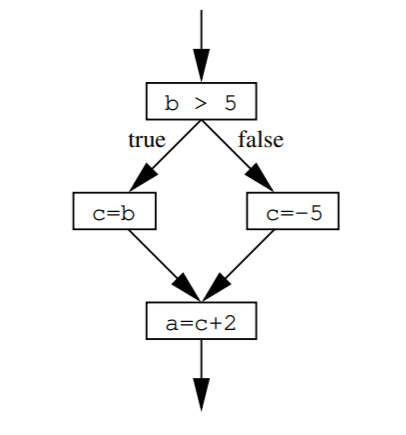
\includegraphics[width=0.8\textwidth]{img/2.png}
	\end{columns}
\end{frame}

%------------------------------------------------

\begin{frame}[fragile]{Abstract States}
	\note{Instead of having an abstract state for each line of code like before, we have
		an abstract state for each node in the CFG.}

	\begin{columns}[c] % The "c" option specifies centered vertical alignment while the "t" option is used for top vertical alignment

		\column{.45\textwidth} % Left column and width

		\begin{itemize}
			\item Recall: each element of the lattice {\it State = Var $\rightarrow$ Sign} is an
			      abstract state that maps variables to signs
			\item For each CFG node $v$, let the {\bf constraint variable} $[[v]]$ be the abstract state at the program point {\it
					      immediately after} $v$
			\item We have a lattice $\textit{State}^{n}$ of abstract states, where $n$ is the
			      number of CFG nodes
		\end{itemize}

		\column{.45\textwidth} % Right column and width
		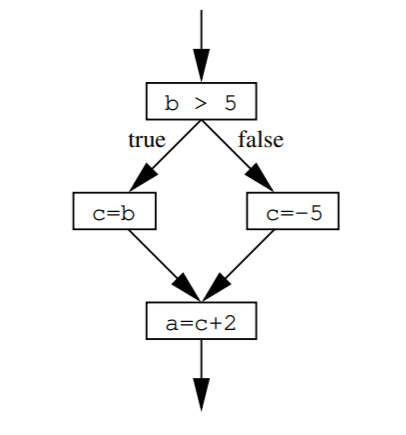
\includegraphics[width=0.8\textwidth]{img/2.png}
	\end{columns}
\end{frame}

%------------------------------------------------

\begin{frame}[fragile]{Constraint Rules}
	\begin{columns}[c] % The "c" option specifies centered vertical alignment while the "t" option is used for top vertical alignment

		\column{.45\textwidth} % Left column and width

		We need to combine the abstract states of the predecessors of a node to get the
		abstract state of the node itself.

		\[
			\text{JOIN}(v) = \bigsqcup_{u \in \text{pred}(v)} [[u]]
		\]

		\column{.45\textwidth} % Right column and width
		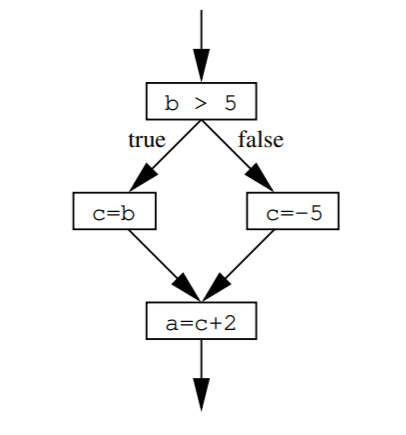
\includegraphics[width=0.8\textwidth]{img/2.png}
	\end{columns}

	$$\text{JOIN}([[a=c+2]]) = [[c=b]] \sqcup [[c=-5]]$$
\end{frame}

%------------------------------------------------

\begin{frame}[fragile]{Constraint Rules}
	\note{After $c=b$, we know both $b$ and $c$ are positive, since $b$ is positive in
		the control flow}
	\note{After $c=-5$, we know $c$ is negative, but we don't know anything about $b$}
	\note{So when joining them, we really don't know anything about $b$ or $c$}
	\note{The sign of $a$ depends on the result of evaluating $c+2$, with the context
		of the abstract state at that point.}
	\note{Because we don't know anything about $b$ or $c$, we don't know anything about
		$a$ either.}

	\begin{columns}[c] % The "c" option specifies centered vertical alignment while the "t" option is used for top vertical alignment

		\column{.45\textwidth} % Left column and width

		\begin{align*}
			 & [[c=b]]  & = [b \mapsto +, c \mapsto +]    \\
			 & [[c=-5]] & = [b \mapsto \top, c \mapsto -] \\
		\end{align*}
		\begin{align*}
			\text{JOIN}([[a=c+2]]) & = [[c=b]] \sqcup [[c=-5]]          \\
			                       & = [b \mapsto \top, c \mapsto \top]
		\end{align*}

		\column{.45\textwidth} % Right column and width
		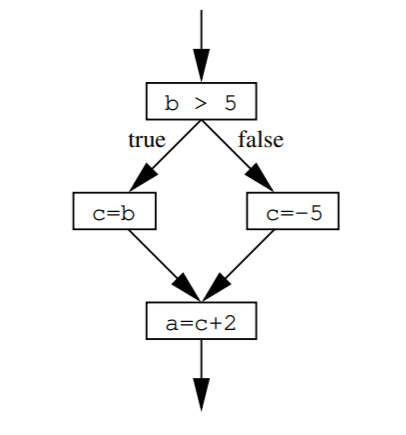
\includegraphics[width=0.8\textwidth]{img/2.png}
	\end{columns}

	\begin{align*}
		[[a=c+2]] & = \text{JOIN}([[a=c+2]])[a \mapsto eval(JOIN([[a=c+2]]), c+2)] \\
		          & = [a \mapsto \top, b \mapsto \top, c \mapsto \top]
	\end{align*}
\end{frame}

%------------------------------------------------

\begin{frame}{Solving Data Flow Equations}
	\note{Same as what we did before, but with the constraint variables representing the
		abstract states of the CFG nodes.}

	Generalised equation system over a lattice $L$, with functions $f_i: L^n
		\rightarrow L$:
	\begin{align*}
		[[v_1]] & = f_{v_1}([[v_1]], \ldots, [[v_n]]) \\
		[[v_2]] & = f_{v_2}([[v_1]], \ldots, [[v_n]]) \\
		\vdots                                        \\
		[[v_n]] & = f_{v_n}([[v_1]], \ldots, [[v_n]])
	\end{align*}

	Combine the $n$ functions into $F: L^n \rightarrow L^n$:
	\begin{align*}
		F([[v_1]], \ldots, [[v_n]]) & = (f_{v_1}([[v_1]], \ldots, [[v_n]]), \ldots, f_{v_n}([[v_1]], \ldots, [[v_n])) \\
		                            & = ([[v_1]], \ldots, [[v_n]])
	\end{align*}

	Then we are looking for $x = F(x)$, i.e. a fixed point of $F$.
\end{frame}

%------------------------------------------------

\begin{frame}[fragile]{A More Efficient Algorithm}
	\begin{columns}[c] % The "c" option specifies centered vertical alignment while the "t" option is used for top vertical alignment

		\column{.45\textwidth} % Left column and width

		\begin{algorithm}[H]
			\footnotesize
			\begin{algorithmic}[1]
				\Procedure{SimpleWorkList}{$F$}
				\State $(x_1, \ldots, x_n) := (\bot, \ldots, \bot)$
				\State $W := \{v_1, \ldots, v_n\}$
				\While{$W \neq \emptyset$}
				\State $v_i := W.\text{pop}()$
				\State $y := f_{v_i}(x_1, \ldots, x_n)$
				\If{$y \neq x_i$}
				\State $x_i := y$
				\For{$v_j \in \text{dep}(v_i)$}
				\State $W.\text{add}(v_j)$
				\EndFor
				\EndIf
				\EndWhile
				\State \Return $(x_1, \ldots, x_n)$
				\EndProcedure
			\end{algorithmic}
			\caption{Simple Worklist Algorithm}
		\end{algorithm}

		\column{.45\textwidth} % Right column and width

		Insight: most $f_{v_i}$ will only read the values from a few other variables,
		instead of all $[[v_1]], \ldots, [[v_n]]$.

		\bigskip

		$dep(v_i)$ is the set of nodes that depend on $v_i$ (i.e. the successors of $v_i$)
	\end{columns}
\end{frame}

%------------------------------------------------

\begin{frame}{Taint Tracking}
	\begin{itemize}
		\item {\bf Can we tell which computations may involve ``tainted'' data?}
		\item i.e. data that comes from an untrusted source
		\item e.g. user input, HTTP responses, environment variables
	\end{itemize}
\end{frame}

%------------------------------------------------

\begin{frame}{Taint Tracking}

	The approach is similar! We just define different abstract values and
	equations. \bigskip

	\begin{itemize}
		\item \textbf{Abstract taint values}:
		      \begin{itemize}
			      \item $\top$: Unknown taint status.
			      \item $T$: Tainted.
			      \item $U$: Untainted.
			      \item $\bot$: Unreachable.
		      \end{itemize}
		\item \textbf{Ordering:} $\bot \sqsubseteq U \sqsubseteq T \sqsubseteq \top$
		\item \textbf{Abstract state:} A mapping $\sigma: \text{Var} \rightarrow \{ \bot, U, T, \top \}$.
		\item \textbf{Transfer functions:}
		      e.g. for an assignment $x := y\ \texttt{op}\ z$, define
		      \[
			      f(\sigma) = \sigma[x \mapsto \sigma(y) \sqcup \sigma(z)]
		      \]

		      i.e. if either operand is tainted, the result is tainted
	\end{itemize}
\end{frame}

%------------------------------------------------
\section{CodeQL}
%------------------------------------------------

\begin{frame}{In Practice: CodeQL}

	A tool developed by Semmle (a spin-out company from Oxf*rd), now acquired by
	GitHub. Used with CLI or GitHub integration (free for all public repos!)
	\bigskip

	\begin{itemize}
		\item The source code is compiled into a relational database, which includes
		      information about the control flow graph, data flow, and other properties of
		      the code.
		\item The user writes queries in a high-level language called QL, which is executed
		      by the CodeQL engine.
		\item The engine uses fixed-point algorithms to perform data flow analysis.
		\item Results are exported into the SARIF format which can be consumed by CI tools or
		      custom integrations.
	\end{itemize}
\end{frame}

%----------------------------------------------------------------------------------------
\begin{frame}[fragile]{Let's Go On A Little Adventure}
	\begin{itemize}
		\item Next.js, the most popular React framework, has some weird, poorly documented
		      URL parsing semantics that does not conform to the widely accepted WHATWG URL
		      standard
		\item This is unexpected behaviour, and often results in wrong URL validation
		\item Made a responsible disclosure $\approx 1$ year ago, still not fixed \end{itemize}
	\bigskip
	Let's query open-source GitHub projects to find instances of this bug!
	\bigskip
	\begin{itemize}
		\item Common design pattern: unauthenticated user visits \verb|/admin|, gets
		      redirected to \verb|/login?next=/admin|, logs in, and gets redirected back to
		      \verb|/admin|
		\item Use Next.js URL parsing trickery to turn a ``normal'' URL into
		      \verb|javascript:sendToAttacker(authToken)| at the final step
	\end{itemize}
\end{frame}

%----------------------------------------------------------------------------------------
\begin{frame}{Taint Tracking in CodeQL}
	We want to find all instances where untrusted user input (source) reaches a
	sensitive function (sink) without being sanitized.

	\begin{figure}
		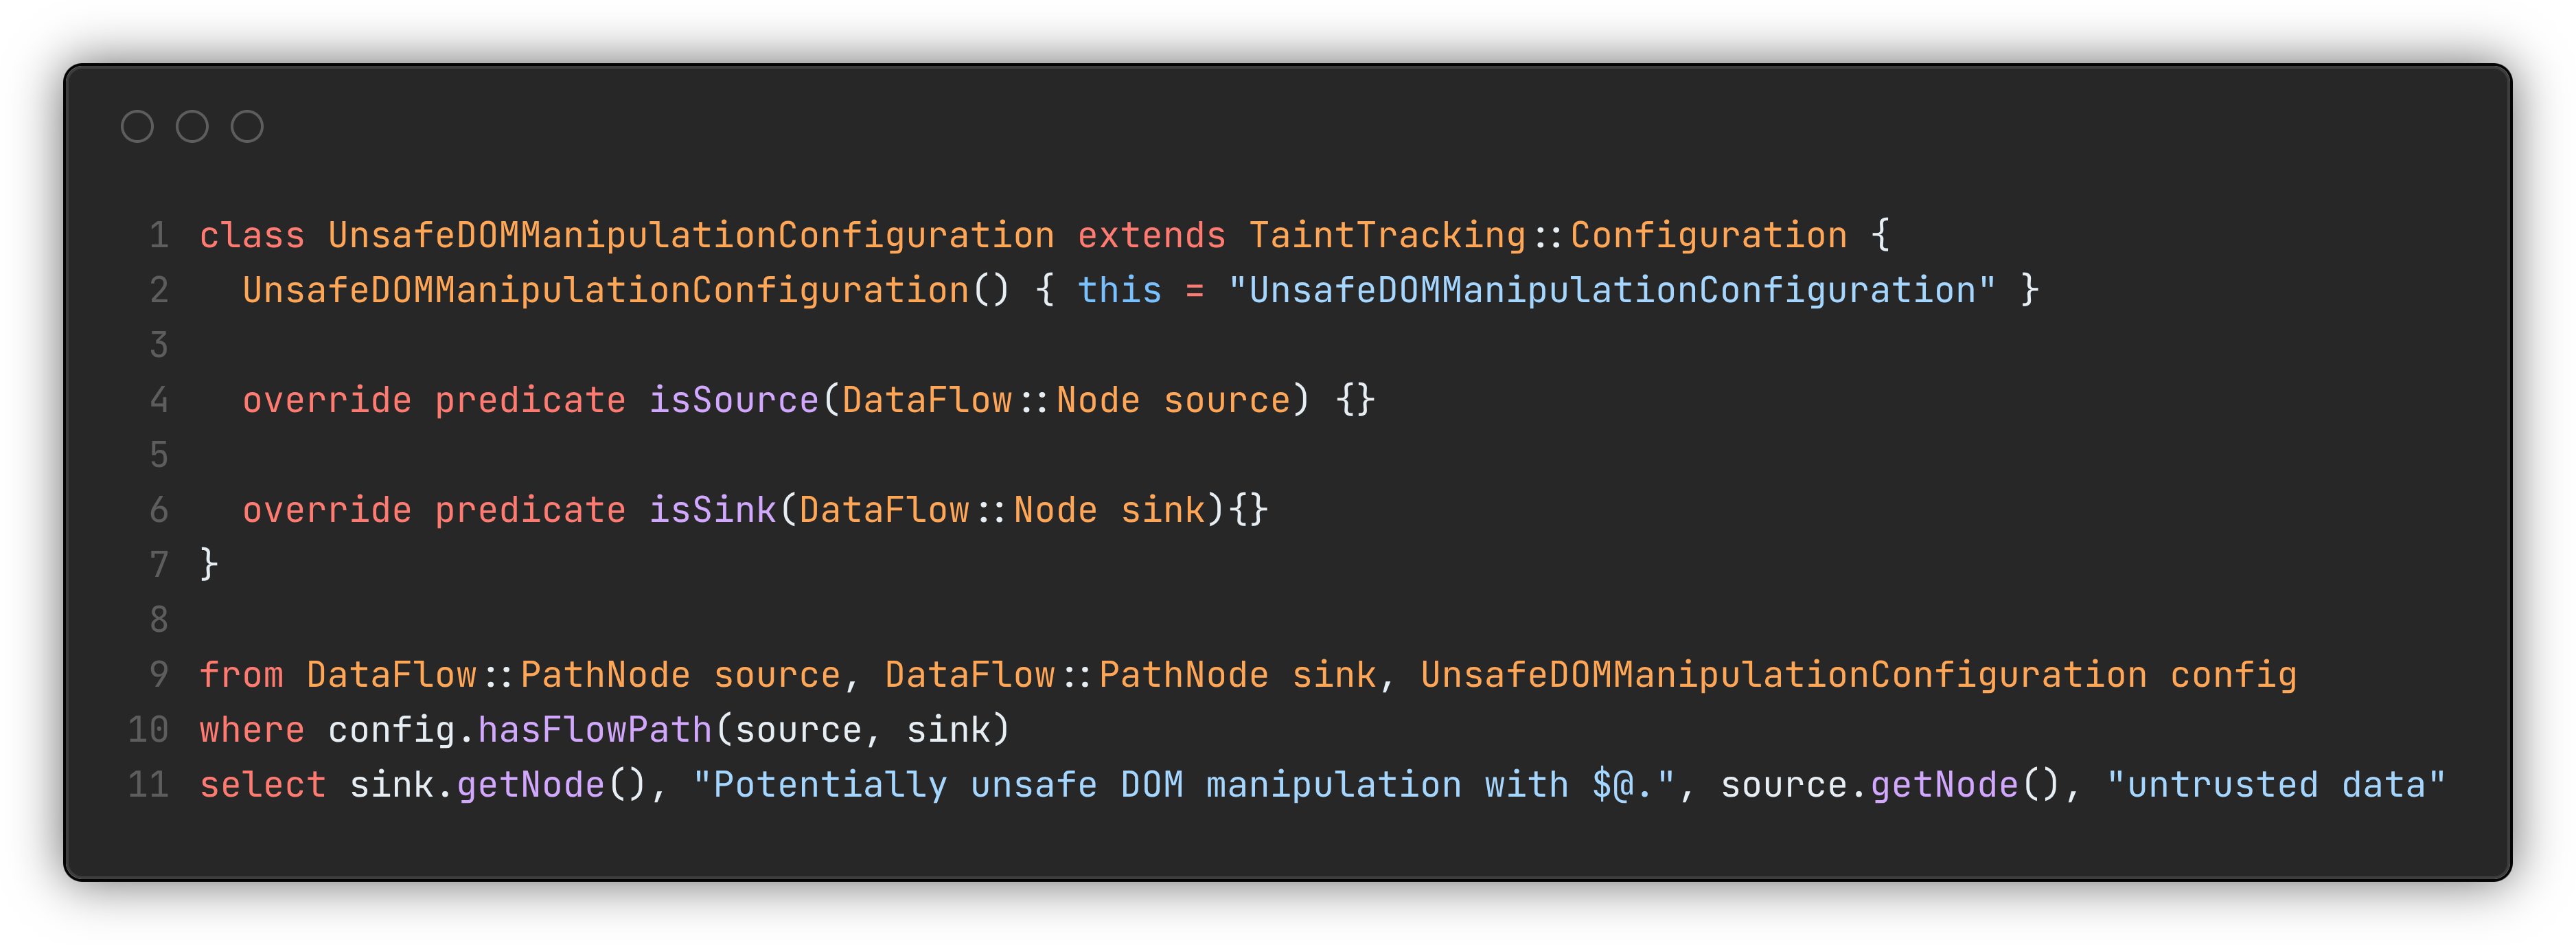
\includegraphics[height=0.7\textheight]{img/3.png}
	\end{figure}
\end{frame}

%----------------------------------------------------------------------------------------
\begin{frame}{Defining Sources}

	\begin{figure}
		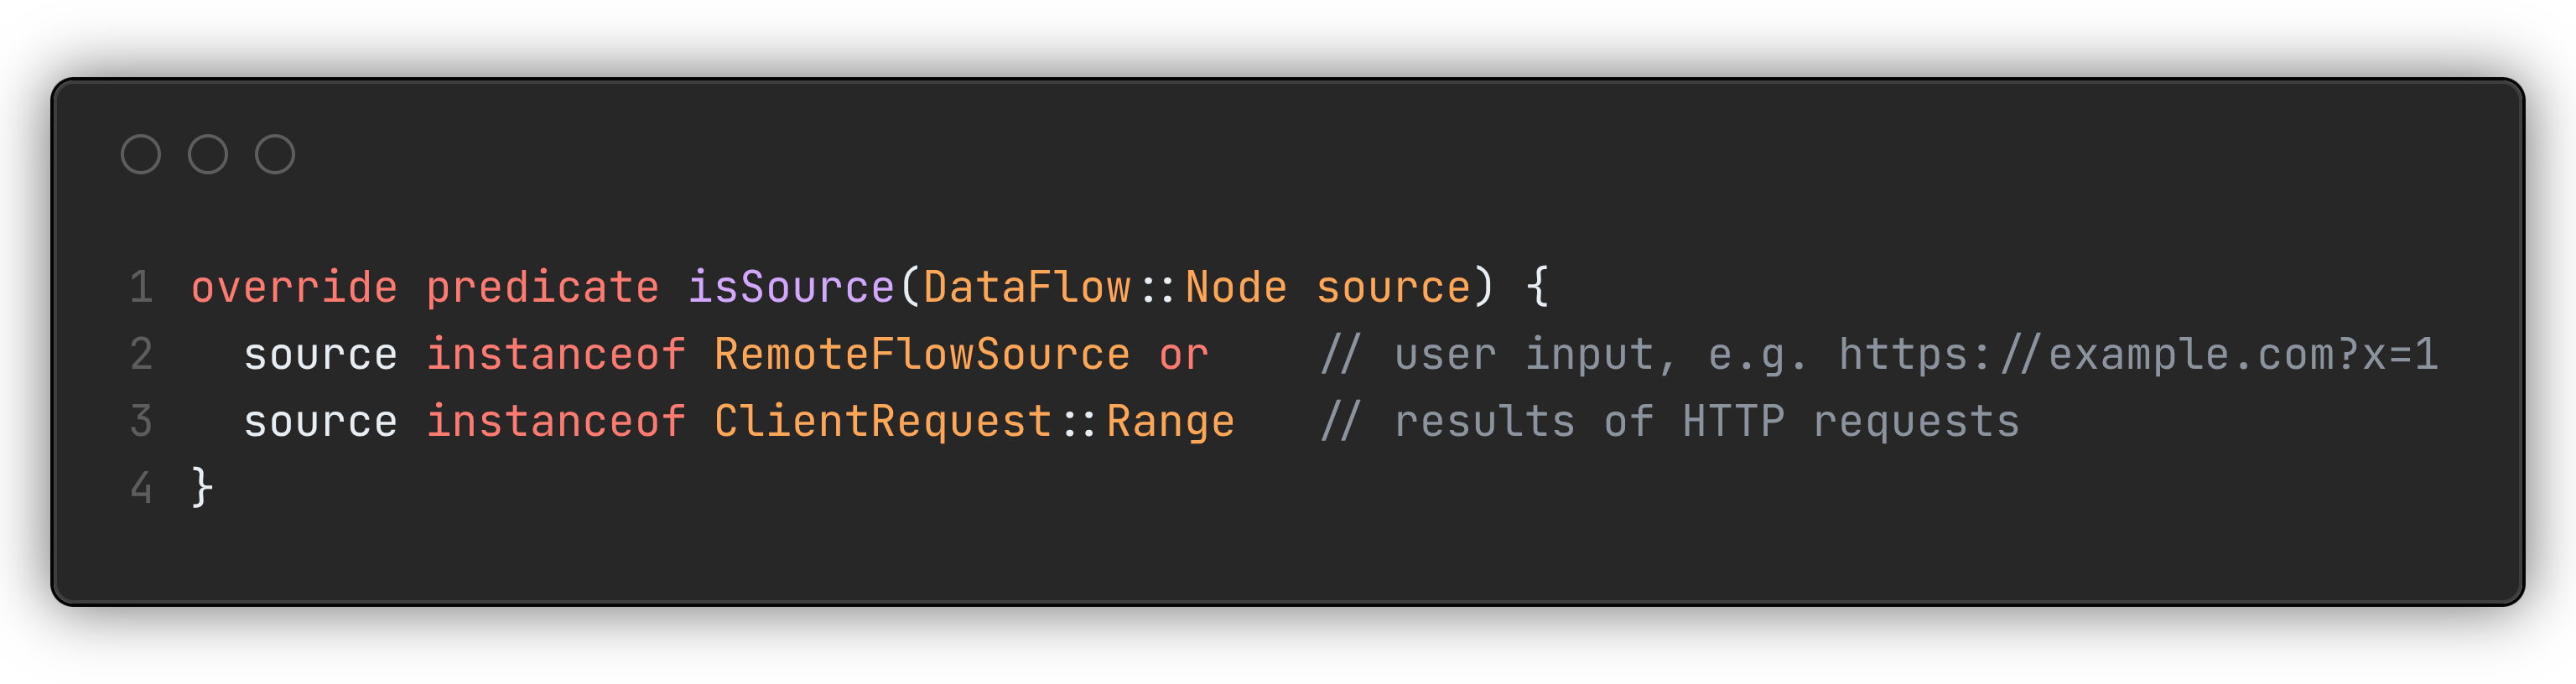
\includegraphics[width=\textwidth]{img/4.png}
	\end{figure}

	You can also extend this with custom logic, to incorporate codebase-specific
	patterns

	e.g. RPC calls, deserialization, etc.

\end{frame}

%----------------------------------------------------------------------------------------
\begin{frame}{Defining Sinks}

	\begin{figure}
		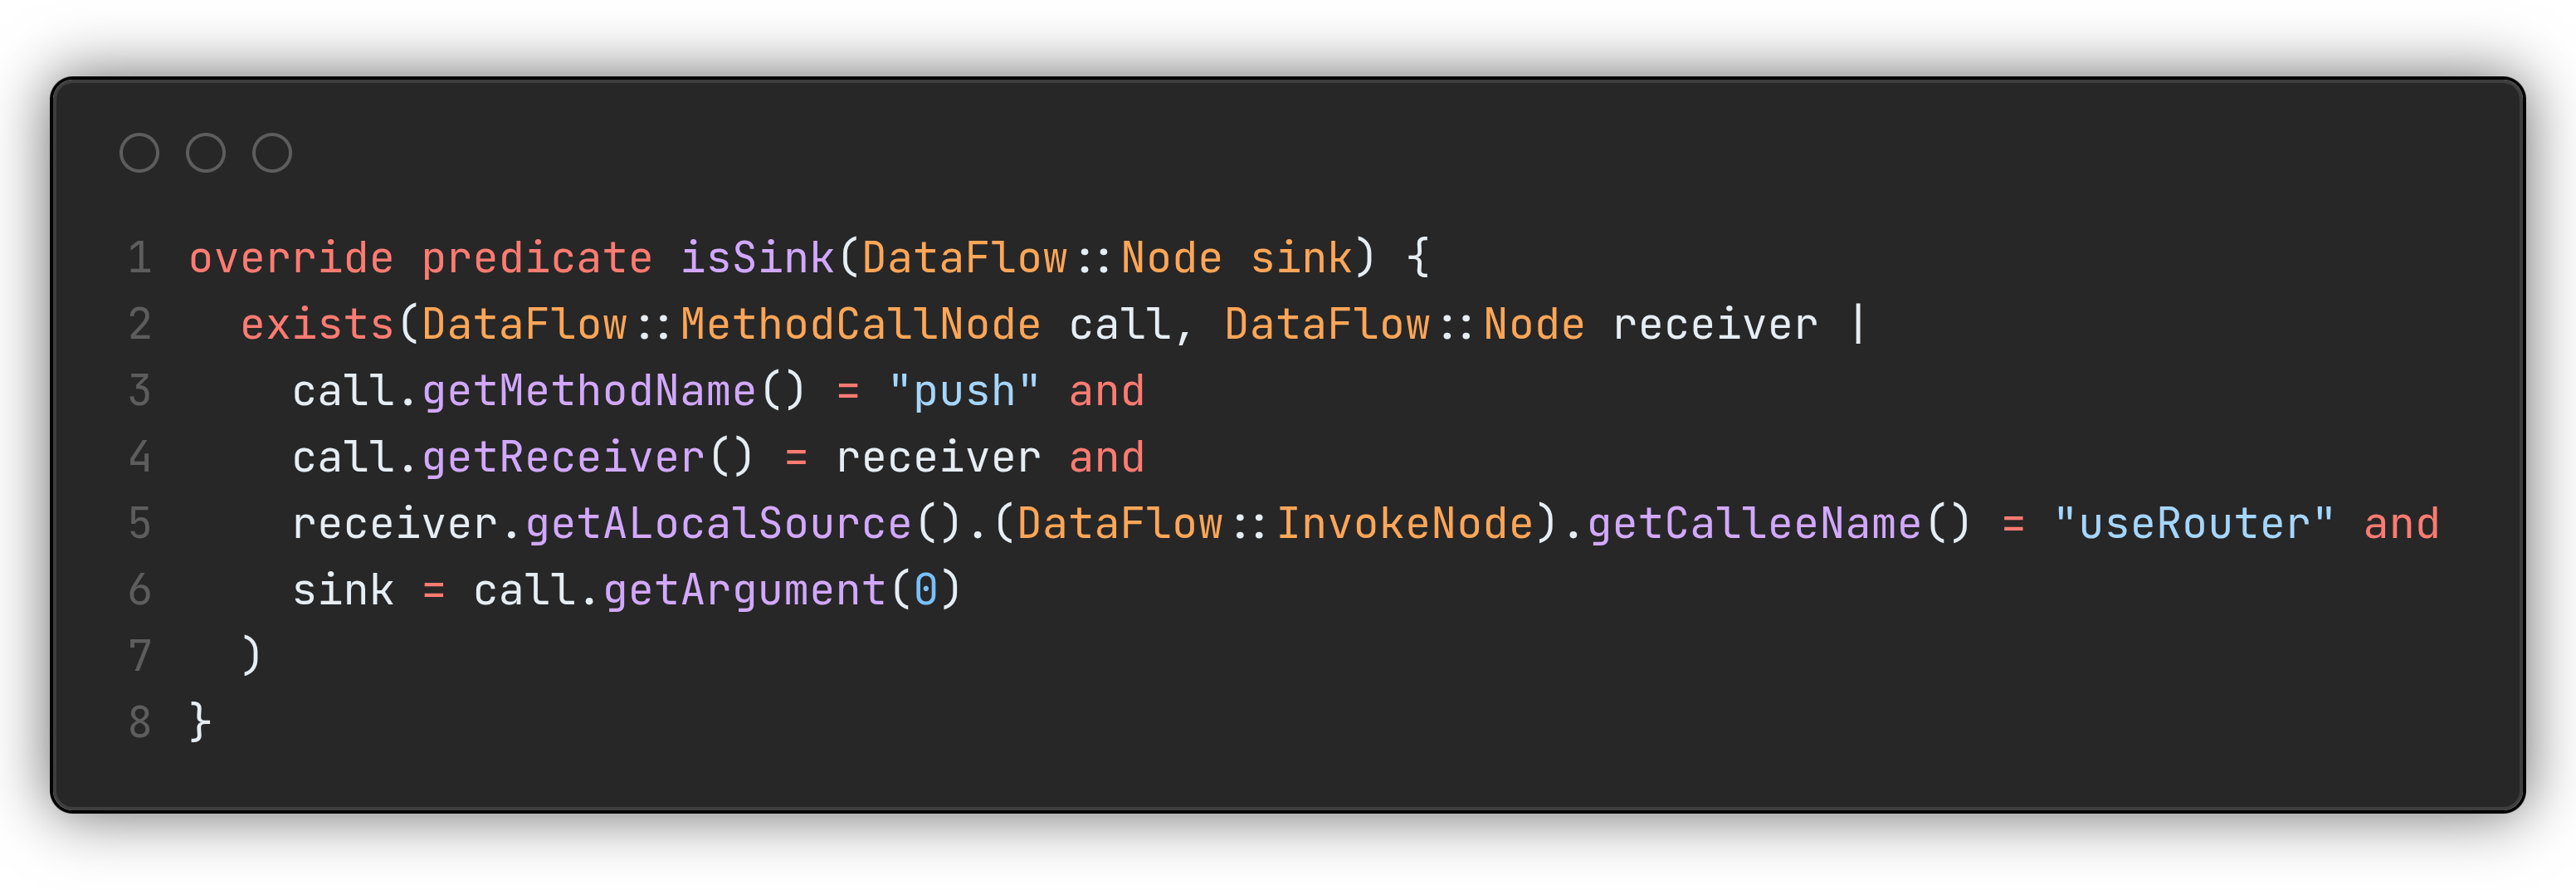
\includegraphics[width=\textwidth]{img/5.png}
	\end{figure}
	\vspace{-1em}
	\begin{align*}
		\text{isSink}(\text{node}) \triangleq \  & \exists \ \text{call}, \text{receiver} \ .\   \text{call invokes the {\bf.push} method on receiver} \ \land                           \\
		                                         & \exists \ \text{invocation} \ .\   \text{invocation is {\bf useRouter()}} \land \text{invocation} \rightarrow^* \text{receiver} \land \\ \
		                                         & \text{node} = \text{{\bf args}(call)[0]}
	\end{align*}
\end{frame}

%----------------------------------------------------------------------------------------
\begin{frame}{Changing the Transfer Function}

	\begin{figure}
		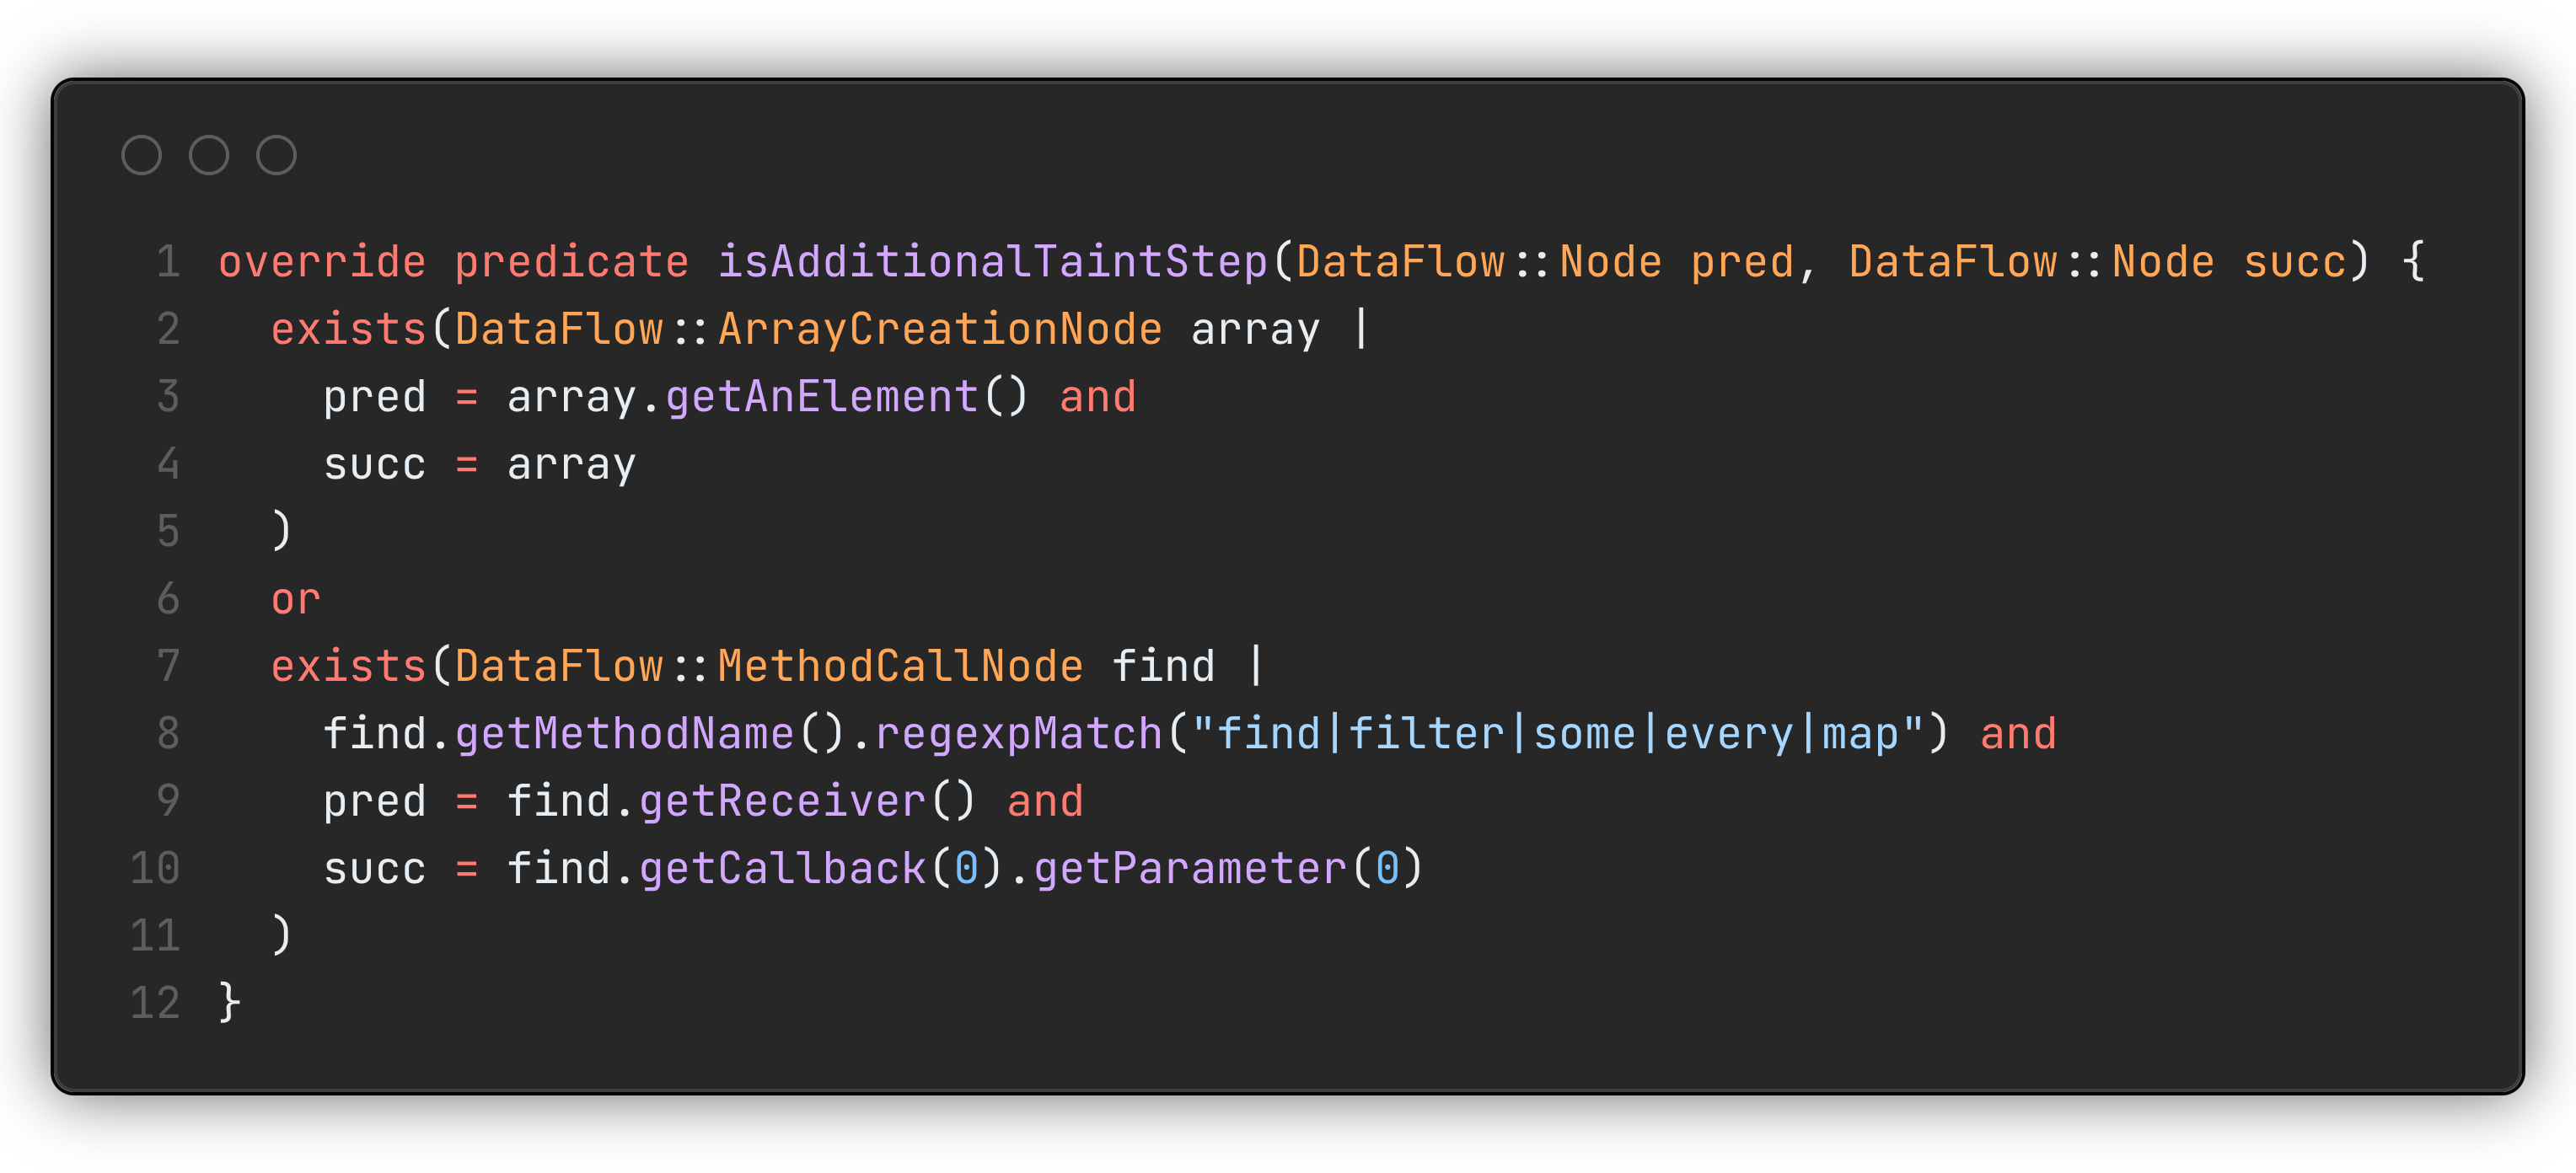
\includegraphics[width=\textwidth]{img/6.png}
	\end{figure}
\end{frame}

%----------------------------------------------------------------------------------------
\begin{frame}{Changing the Transfer Function}

	\begin{figure}
		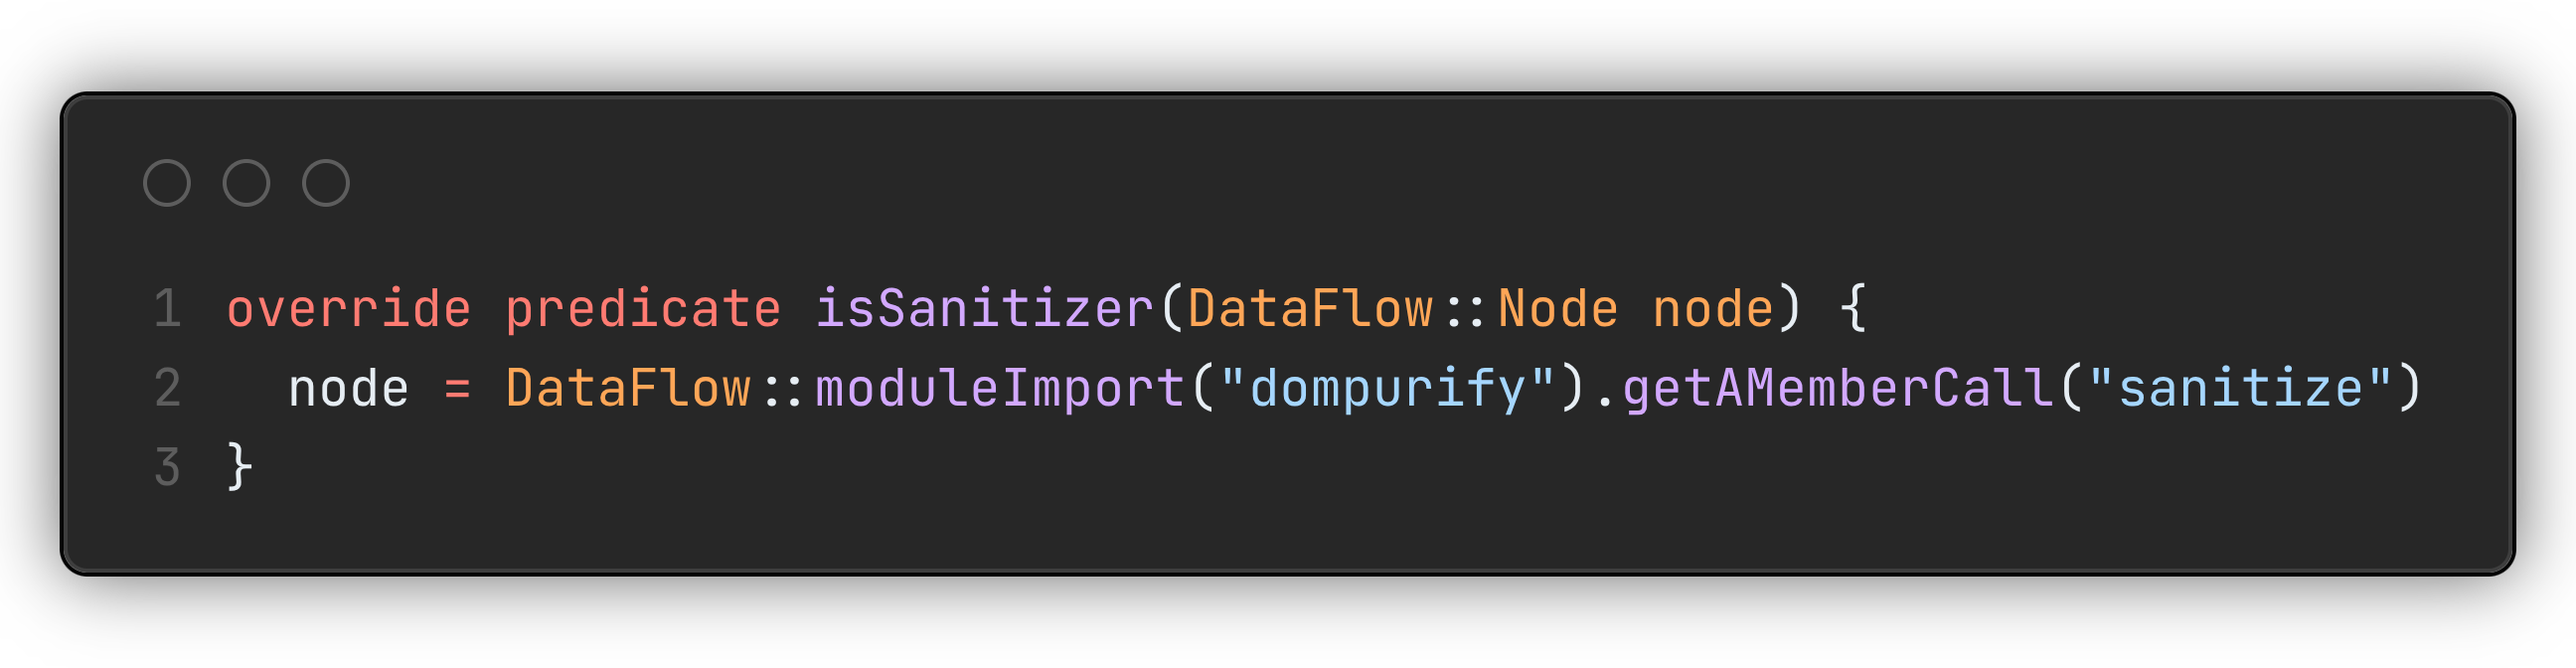
\includegraphics[width=\textwidth]{img/7.png}
	\end{figure}

	Any results from DOMPurify.sanitize are treated as untainted. Know your
	assumptions!
\end{frame}

%----------------------------------------------------------------------------------------
\begin{frame}{Let's Go Hunting}

	\begin{figure}
		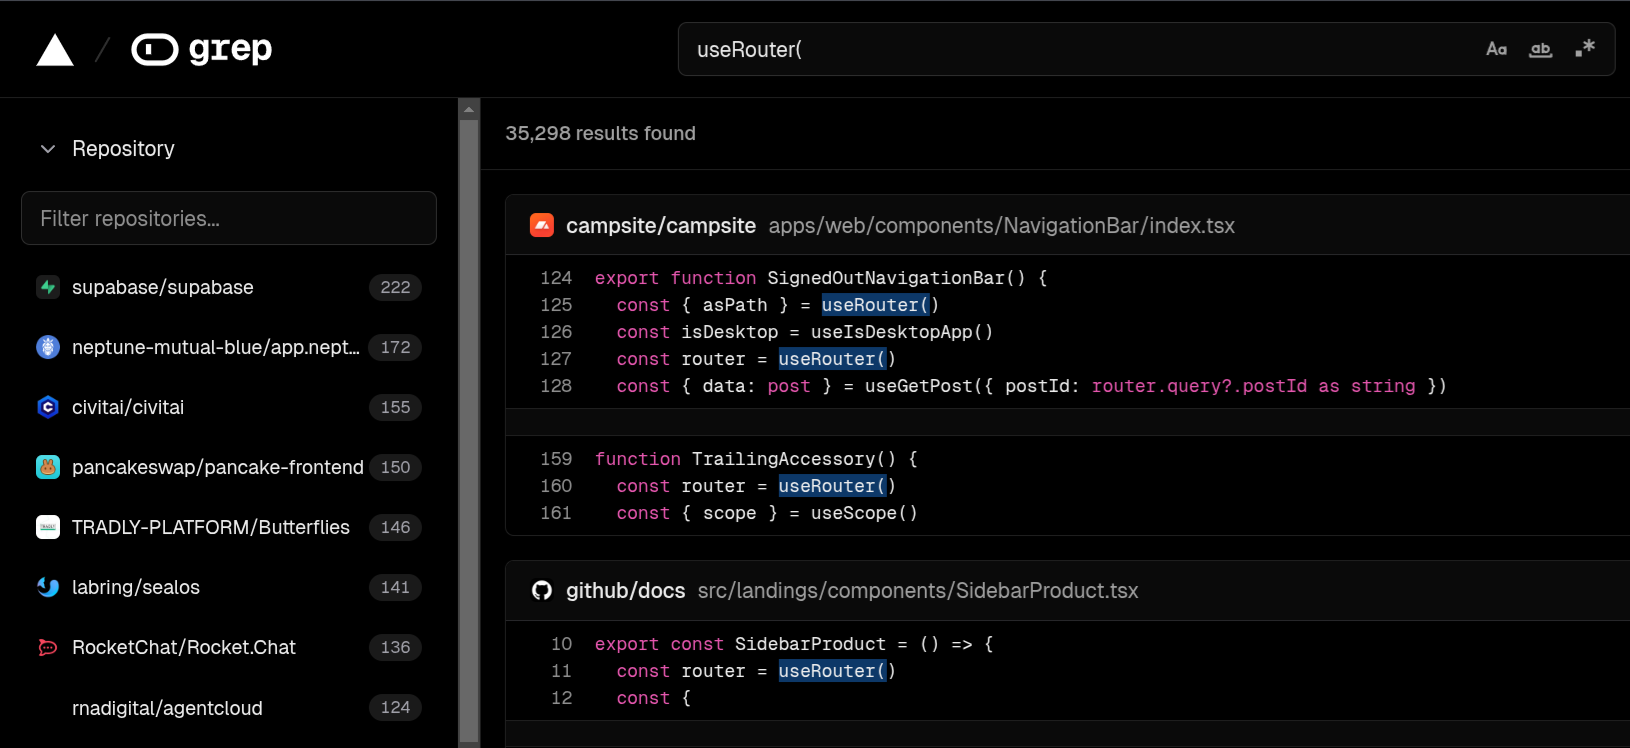
\includegraphics[width=\textwidth]{img/8.png}
	\end{figure}

\end{frame}

%----------------------------------------------------------------------------------------
\begin{frame}{Let's Go Hunting}
	\note{Begin demo here. Show the variant analysis results on VSCode, and show the demo exploit.}
	\begin{figure}
		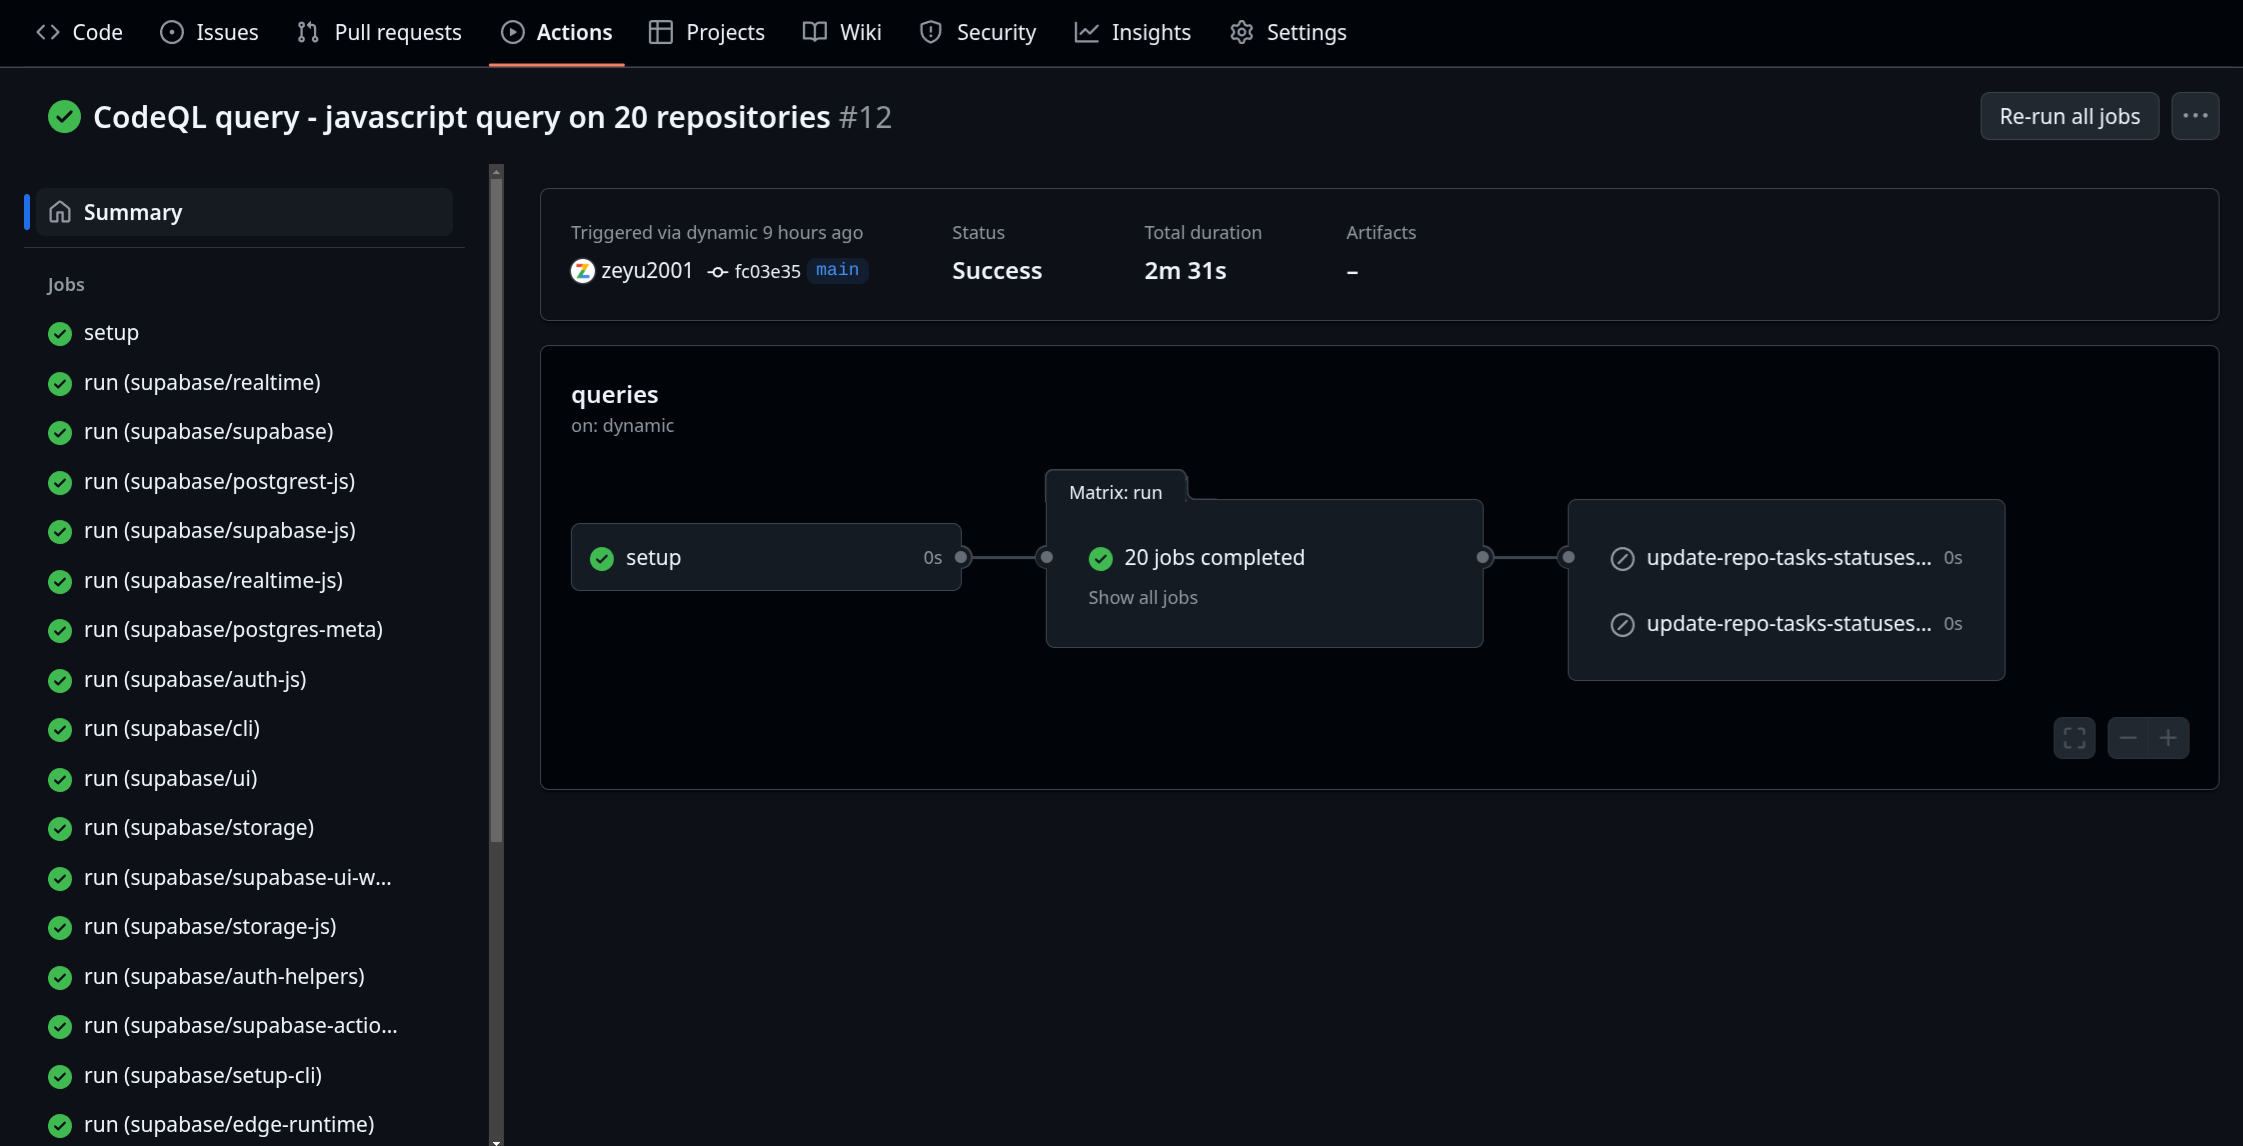
\includegraphics[height=0.75\textheight]{img/9.png}
	\end{figure}

\end{frame}

%----------------------------------------------------------------------------------------
\begin{frame}{Limitations}

	CodeQL is very useful as a CI integration to catch security issues early in the
	development process, and provide guarantees about your code. But it's really
	hard to get right \dots

	\bigskip

	\begin{itemize}
		\item We need to create custom taint specifications for third-party library APIs.
		\item False positives: even if tainted data reaches a sink, it may not always be
		      exploitable -- some other conditions may need to be met
		\item Requires a good understanding of the codebase and the problem domain, and lots
		      of fine-tuning to get good results -- only as good as the queries you write
	\end{itemize}
\end{frame}

%----------------------------------------------------------------------------------------
\begin{frame}{Alternative Approaches}

	\begin{itemize}
		\item {\bf Symbolic execution}: represent the program inputs symbolically and explore all
		      possible paths through the program, generating constraints on the inputs such
		      that a certain path is taken
		\item Ziyang Li, Saikat Dutta, and Mayur Naik. LLM-assisted static analysis for
		      detecting security vulnerabilities, 2024 \bigskip

		      \begin{quote}
			      IRIS leverages LLMs to infer taint specifications and perform contextual analysis, alleviating needs for human specifications and inspection \dots

			      A state-of-the-art static analysis tool CodeQL detects only 27 of these
			      vulnerabilities whereas IRIS with GPT-4 detects 55 (+28) and improves upon
			      CodeQL's average false discovery rate by 5\% points.
		      \end{quote}
	\end{itemize}
\end{frame}

%----------------------------------------------------------------------------------------

\begin{frame}{References}
	\nocite{*}
	\bibliographystyle{unsrt}
	\bibliography{refs} % Entries are in the refs.bib file
\end{frame}

\end{document}